\section{Systemdesign}
\subsection{Navigasjon}
\subsubsection{Struktur og oppdeling}
Appen består av to hovedelementer for navigasjon, et bottom-navigation element, og et navigation-drawer element. I tillegg til disse har den en swipe-funksjon som gjør det mulig å åpne navigation-drawer. Det vil være mulig å navigere mellom disse tre sidene med bottom-navigation elementet. Det vil være en navigation-drawer tilgjengelig fra alle sider bortsett fra innloggingssiden som brukes til å navigere til resten av appen.

Grunnen til denne oppdelingen er for å skille mellom sider som blir brukt mye og sider som blir brukt lite. Vi har valgt å bruke bottom-navigation og swipe-funksjonen til forsiden, kartsiden og vennesiden, fordi de er sentrale og brukes nesten hver gang appen er i bruk. Forsiden er det samme som oversiktssiden, så dette vil være landingssiden når brukeren logger inn. I navigation-drawer elementet kan man blant annet navigere seg til innstillinger og enhetskatalogen.

\subsubsection{Navigation Pattern}
Som hurtig navigasjon mellom de viktigste sidene bruker vi bottom-navigation og navigation-drawer. Disse er to gode navigasjons-verktøy fra navigation-pattern som kalles "Literal navigation" siden man velger direkte hvor man ønsker å navigere. Vi har også inkludert forwards navigation i form av knappene i oversiktssiden og vennesiden. For eksempel vil pluss-knappen i oversiktssiden navigere brukeren til drikke-katalogen. Til slutt bruker vi backwards-navigation i form av en pil tilbake som fører brukeren til sist besøkte side.

\subsubsection{Navigasjonsflyt}

\begin{figure}[H]
    \centering
    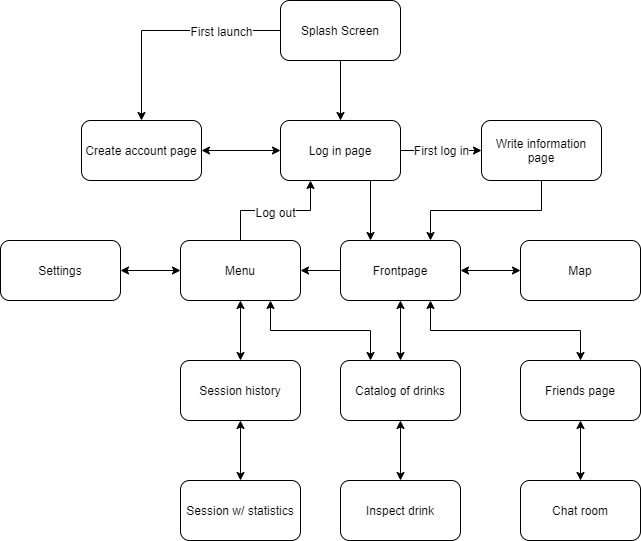
\includegraphics[scale=0.5]{images/lille_promille_float_diagram.drawio.png}
    \caption{Diagrammet viser hvor man kan navigere seg til fra hvilke sider i appen.}
\end{figure}

\begin{figure}[H]
    \centering
    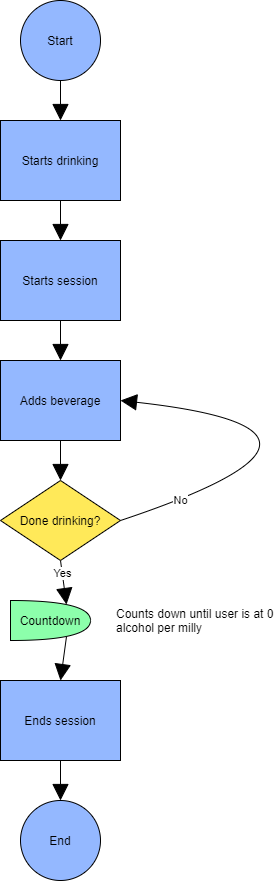
\includegraphics[scale=0.4]{images/lille_promille_user_float.drawio.png}
    \caption{Diagramet viser hvordan bruker vanligvis vil samhandle med appen.}
\end{figure}

\subsection{Teknisk oppbygging}
\subsubsection{Services}
Det kan være behov for services. Blant annet skal vi implementere gps-sporing og push-notifikasjoner, i tillegg til bør nedtellingsklokken i en økt telle ned mens appen ikke er i bruk. Foreløpig tenker vi at mye kan løses via threads og asynce funksjoner, derfor er vi usikre på om det er behov for services i det hele tatt.

\subsubsection{Fragmenter}
I vår app er fragmenter et behov. Siden vi bruker Navigation Component biblioteket, er det best praksise å bytte ut sidene via fragmenter. Vi har derfor delt opp appen i tre aktiviteter, hvor vi bytter ut fragmenter i hver av aktivitetene. Dette er både for å gjøre koden mer lesbar ved å abstrahere i logiske inndelinger og for å skille på de forskjellige navigasjonsmetodene, siden bottom-navigation og navigation-drawer kun finnes i hovedaktiviteten.

\subsubsection{Lagring og uthenting av data}
For å lagre brukerdata benyttes Firestore. Dette gjøres via Firebase, her lagres brukere i en "user" collection. Hver bruker lagres med en UUID som autogeneres fra Firebase. 

Brukerinformasjonen lagres rett i dokumentet til brukeren, mens enhetskatalogen og økthistorikken lagres i collections på brukeren. 

Når en bruker logger inn hentes dataen til brukeren ved å bruke Firebase UUID'en, da oppdateres først dokumentreferansen så brukes denne til å hente riktig data, brukerdaten blir da lagret i et repository, denne dataen hentes da senere i settingsFragment via et ViewModel. 

Når brukeren logger inn gjøres det en sjekk på om det er en ny bruker, hvis det er en ny bruker hentes ikke dataen. 
Da legges det til en bruker med tomme verdier til database. 

Når brukeren navigerer ut av settingsFragment hentes den oppdaterte dataen fra Firebase.

\subsubsection{Brukerhåndtering}
Håndtering av brukere gjøres gjennom Firebase.

Brukeren får via appen muligheten til å lage en ny bruker, oppdatere og slette brukeren.

En bruker består av feltene:
\begin{itemize}
    \item age
    \item height
    \item weight
    \item gender
    \item username
    \item currentSession
    \item weight
\end{itemize}

En sessionHistory collection og en alcoholUnitCollection.

\subsection{Ressurser}

\subsubsection{Klasser}
Ekskluderer klasser relatert til aktiviteter og fragmenter, består appen av modell-klasser og referanse-klasser. Modellen består av følgende klasser:

\begin{tabular}{ | m{4cm} | m{12cm} | } 
    \hline
    \textbf{Klassenavn} & \textbf{Beskrivelse} \\
    \hline
    AlcoholUnit &
    Representerer en enhet som blir lagt til i en økt, arver fra beverage \\
    \hline
    Beverage &
    Representerer en drikke \\
    \hline
    Settings &
    Håndterer app-innstillinger \\
    \hline
    Session &
    Representerer en økt, og har relaterte metoder \\
    \hline
    SessionLimit &
    Definerer en grense på hvor mye man ønsker å drikke i en økt (session) \\
    \hline
    User &
    Definerer en bruker og inkluderer relaterte variabler \\
    \hline
\end{tabular}

I tillegg har vi klasser for å data fra firestore. Disse ligger i en mappe kalt Datahandler, og inkluderer disse klassene:

\begin{tabular}{ | m{4cm} | m{12cm} | } 
    \hline
    \textbf{Klassenavn} & \textbf{Beskrivelse} \\
    \hline
    BeverageCatalogHandler &
    Håndterer data relatert til drikke-katalogen i appen \\
    \hline
    Beverage &
    Hånterer brukerdata \\
    \hline
\end{tabular}

\subsubsection{Bilder}
Bilder i appen vil bestå av ikoner, logoer, emojier og eventuelt profilbilder. Ikonene brukes til å veilede brukeren der det er raskere å oppfatte ikonet enn å det er å lese teksten, for eksempel til navigasjonspunktene i bottom-navigation og navigation-drawer. Ikonene er en blanding av lånte og egenskapte ikoner som følger design prinsippene til Material Design dokumentasjonen(1). For eksempel at ikonet skal være uthevet og tydelig.

Lille promille logoen har vi designet og laget selv. Det vil også være flere versjoner av logoen til de forskjellige seksjonene i appen der det er passende. For eksempel i sprutskjermen viser den hele logoen, som inkluderer teksten, mens i appikonet bruker den en minimalisert versjon av logoen.

I vennesiden brukes emojier til å visualisere hvilken alkoholstatus vennene har. Vi tror dette er en smart løsning fordi mange brukere er allerede familiære med systemet som Snapchat bruker, hvor de forklarer forholdet man har til en venn. Til denne funksjonen bruker Lille promille standardemojiene til android.

Hvis ønskelig kan brukeren legge til sitt eget profilbilde i innstillingene. Dette profilbilde vises både i navigation-drawer ved brukernavnet og i vennesiden ved siden av navnet sitt. Bildet kan hentes fra kamerarullen eller kan tas direkte fra kameraet.

\subsubsection{Lyd}
Dette har vi ikke tenkt på hittil.

\subsubsection{Biblioteker}

\begin{itemize}
    \item Firestore (Firebase) - Dokumentdatabase for lagring av data
    \item Google dependency - Gir mulighet for innlogging Google-bruker
    \item Navigation Component - Brukes til all navigasjon innad i appen
    \item JUnit - Bibliotek for enhets-testing
    \item Google Play Location - For mobil-sporing
\end{itemize}

\subsubsection{Hva vi er usikre på}
Vi må implementere threads på henting av data, dette er vi ganske usikre på hvordan vi skal gjøre. Vi har enda ikke sett noe på vennefunksjonene og kommer nok til å bruke ganske mye tid på dette. Vi har ikke helt funnet ut av hvordan vi skal regne ut den nåverende promillen dynamisk. AlcoholUnit arver også fra Beverage, dette er fordi vi trenger et sted å lagre når en enhet ble lagret i en session. Vi er litt usikre på om dette er den rette måten å implementere dette på. Vi må også finne ut av hvilke services vi skal bruke og hvordan. Vi har ikke fastslått hvordan vi skal implemetere kartet.